\scanpage{67}\mspage{66}

% The raised inclusion and the continuation have distinct curved connecting strokes.
% Their text is transcribed once, as labels in this drawing.
\figure{%
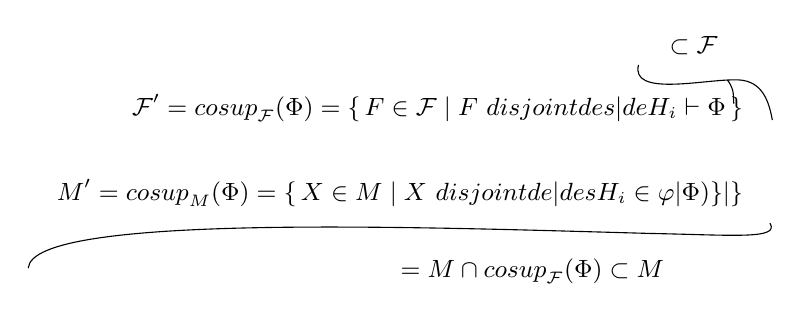
\begin{tikzpicture}[x=1cm,y=1cm,every node/.style={font=\small}]
\node[anchor=base east] (first) at (14.4,0) {$\displaystyle
\mathcal F'=\operatorname{cosup}_{\mathcal F}(\Phi)=
\{\,F\in\mathcal F\mid F\ \text{disjoint \unsure{des|de} }H_i\vdash\Phi\,\}$};
\node[anchor=base] (raised) at (13.65,.78) {$\inserted{\subset\mathcal F}$};
\draw (12.95,.64) .. controls (12.85,.24) and (13.75,.45) .. (14.15,.45)
  .. controls (14.5,.47) and (14.6,.22) .. (14.65,-.06);
\draw (14.08,.45) .. controls (14.18,.31) and (14.15,.23) .. (14.16,.15);
\node[anchor=base east] (second) at (14.4,-1.08) {$\displaystyle
M'=\operatorname{cosup}_{M}(\Phi)=
\{\,X\in M\mid X\ \text{disjoint \unsure{de|des} }H_i\in\unsure{\varphi|\Phi}\unsure{)\}|\}}$};
\node[anchor=base east] (continuation) at (13.4,-2.06) {$\displaystyle
\inserted{=M\cap\operatorname{cosup}_{\mathcal F}(\Phi)\subset M}$};
\draw (14.62,-1.37) .. controls (14.75,-1.58) and (14.15,-1.52) .. (13.1,-1.5)
  .. controls (10.2,-1.42) and (5.25,-1.24) .. (5.2,-1.94);
\end{tikzpicture}%
}

\deleted{Donc \unsure{on aura|on a}, pour $F\in\mathcal F$ posant $\mathcal F'=\operatorname{cosup}_{\mathcal F}$,}

\[
\begin{aligned}
&\deleted{\unsure{\phi|\Phi}}\qquad
\deleted{\mathcal F'=\operatorname{cosupp}_{\mathcal F}(\Phi),\quad M'=\mathcal F'\cap M,}\\[-2pt]
&\qquad\deleted{F\in\operatorname{cosup}_{\unsure{,|\mathcal F}}}
\qquad\qquad\deleted{=\operatorname{cosup}_{\deleted{\unsure{\mathcal F}}M}(\mathcal F)}
\end{aligned}
\]

Donc pour $F\in\mathcal F$

% The left note is slanted. Its arrow and the right note's bent enclosure are drawn.
% These marginal texts occur only here, not again in margin macros.
\figure{%
\begin{tikzpicture}[x=1cm,y=1cm,every node/.style={font=\small}]
\node[anchor=west] (brace) at (4.0,0) {$\displaystyle
\left\{\begin{aligned}
F\in\mathcal F'&\Longleftrightarrow\overline F\subset M'\\
M'&=.\mathcal F'\cap M
\end{aligned}\right.$};
\node[anchor=east,align=left,rotate=13] (leftnote) at (3.35,-.3)
  {Ainsi, $M'$ et $\mathcal F'$\\se \unsure{déterminent|determinent}\\\unsure{mutuellement}};
\draw[->] (3.12,.16) -- (3.75,.26);
\node[anchor=north west,align=left] (rightnote) at (11.0,1.0)
  {NB $\mathcal F',M'$\\sont des\\parties\\fermées de\\$\mathcal F,M$.};
\node[anchor=base west] (familylabel) at (10.3,-1.0) {$\mathcal F'$};
\node[anchor=base west] (stable) at (10.35,-1.51) {\uline{Stable par Sup.}};
\draw[line width=.7pt] (10.3,-1.1) -- (11.12,-1.1) -- (11.12,-.83);
\draw (8.75,-1.24) .. controls (9.5,-1.11) and (9.95,-1.1) .. (10.1,-1.4)
  .. controls (10.18,-1.66) and (12.5,-1.64) .. (13.8,-1.85);
\draw (10.43,-1.13) .. controls (10.05,-1.1) and (10.03,-1.7) .. (10.5,-1.71)
  .. controls (11.9,-1.75) and (13.4,-1.67) .. (14.1,-2.12);
\end{tikzpicture}%
}

Soit d'autre part
\[
\begin{aligned}
\mathcal F''&=\operatorname{cosupp}_{\mathcal F}(\mathcal F')\overset{\text{def}}{=}\operatorname{supp}_{\mathcal F}(\Phi)\\
M''&=\operatorname{cosup}_{M}(\mathcal F')\overset{\text{def}}{=}\operatorname{supp}_{M}(\Phi)
\end{aligned}
\]

On a \unsure{vu|bien|la|là} $\mathcal F''\supset\Phi$, $\mathcal F''$ stable par \unsure{Supp|Sup}, \deleted{contient $\Phi$} et par passage : une sous-figure. Soit $\deleted{\unsure{M}}\overline\Phi=\bigcup_{H_i\in\Phi}\overline H_i$, alors
\[
\begin{aligned}
\operatorname{cosup}_{\mathcal F}(\Phi)&=\operatorname{cosup}_{\mathcal F}(M_{\overline\Phi})\\
\operatorname{cosup}_{\deleted{\unsure{\mathcal F}}M}\unsure{:}(\Phi)&=\{\,\deleted{\unsure{\varnothing|x}}X\in M\mid X\ \text{disjoint de }\unsure{\mathrm{tt}|\forall}\ Y\in M_{\overline\Phi}\,\}
\end{aligned}
\]
donc on est \unsure{ramené|revenu} à des constructions dans $M$. \S

\uline{Partie saturée \inserted{$\mathcal F_0$} de} $\deleted{M}\mathcal F$ : égale au cosupport de son cosupport ($\text{p. r. à }\mathcal F$)\unsure{-|.}

% The short sloping leader belonging to M_0 is retained with its local text.
\figure{%
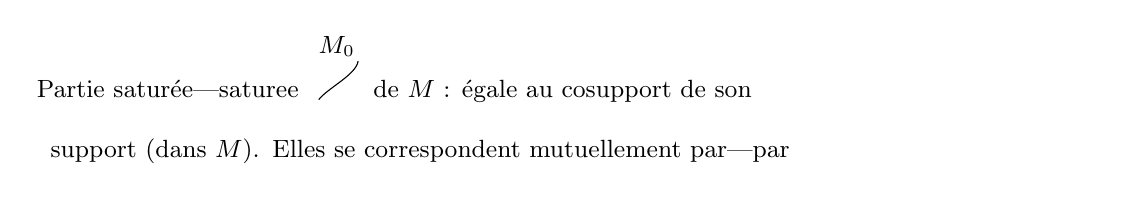
\begin{tikzpicture}[x=1cm,y=1cm,every node/.style={font=\small}]
\node[anchor=base east] at (3.4,0) {Partie \unsure{saturée|saturee}};
\node[anchor=base] at (3.76,.55) {$\inserted{M_0}$};
\draw (4.03,.46) .. controls (4.01,.29) and (3.65,.12) .. (3.53,-.03);
\node[anchor=base west] at (4.1,0) {de $M$ : égale au cosupport de son};
\node[anchor=north west,text width=13.2cm] at (0,-.4)
  {support (dans $M$). Elles se correspondent \unsure{mutuellement} \unsure{par|\deleted{par}}};
\end{tikzpicture}%
}
\[
\begin{aligned}
M_0&=\mathcal F_0\cap M\\
\mathcal F_0&=\{\,F\in\mathcal F\mid\overline F\subset M_0\,\}
\end{aligned}
\]
